\documentclass[a4paper,12pt,final]{report}
\usepackage[margin=0.8in]{geometry}
% Pour une impression recto verso :
%\documentclass[a4paper,11pt,twoside,final]{article}
%%%%% Packages %%%%%
\usepackage[english]{babel}  % Rapport en français
\usepackage[utf8]{inputenc}   % UTF-8 forever <3
\usepackage[T1]{fontenc}      % font encoding (allows accents)
\usepackage[pdftex]{graphicx} % gestion des images
\usepackage{setspace}         % gestion des interlignes
\usepackage{csquotes}         % For quotes
\usepackage[hidelinks]{hyperref}         % gestion des url
\usepackage{titlesec}         % override chapter title
\usepackage{geometry}         % gestion des marges
\usepackage{float}            % Gestion des positionnement d'image
\usepackage[final]{pdfpages}  % Inclusion de fichier pdf
\usepackage{framed}
\usepackage{geometry}
%\usepackage{apacite}

%%% Affichage de code
\usepackage{listings}
\usepackage{xcolor}
\usepackage{textcomp}
% 添加首行缩进,两个字符
\usepackage{indentfirst}
\usepackage[bottom]{footmisc}

\setlength{\parindent}{2em}

\definecolor{comment}{rgb}{0.12, 0.38, 0.18 } % adjusted, in Eclipse: {0.25, 0.42, 0.30 } = #3F6A4D
\definecolor{keyword}{rgb}{0.37, 0.08, 0.25}  % #5F1441
\definecolor{string}{rgb}{0.06, 0.10, 0.98} % #101AF9
\lstset{
  columns=flexible, %prevent extra spaces
  rulecolor=\color{black!50},
  backgroundcolor = \color{blue!10},
  numbers=none, % line numbering
  showspaces=false,
  showtabs=false,
  tabsize=2,
  breaklines=true,
  showstringspaces=false,
  breakatwhitespace=false,
  commentstyle=\color{comment},
  keywordstyle=\color{keyword},
  stringstyle=\color{string},
  basicstyle=\ttfamily,
  extendedchars=true,
  emph=[2]{In},
  emphstyle=[2]\color{black!70},
  morecomment=[l][\color{blue}]{Out},
  frame=single,
  frameround=tttt,
  framerule=0.3pt,
  framesep=4pt,
  belowcaptionskip=2.1pt,
  literate={à}{{\`a}}1 {à }{{\`a} }1 {â}{{\^a}}1 %           letter a
           {À}{{\`A}}1 {Â}{{\^A}}1 %                         letter A
           {ç}{{\c{c}}}1 %                                   letter c
           {Ç}{{\c{C}}}1 %                                   letter C
           {é}{{\'e}}1 {è}{{\`e}}1 {ê}{{\^e}}1 {ë}{{\"e}}1 % letter e
           {É}{{\'E}}1 {È}{{\`E}}1 {Ê}{{\^E}}1 {Ë}{{\"E}}1 % letter E
           {î}{{\^i}}1 {ï}{{\"i}}1 %                         letter i
           {Î}{{\^I}}1 {Ï}{{\"I}}1 %                         letter I
           {ô}{{\^o}}1 %                                     letter o
           {Ô}{{\^O}}1 %                                     letter O
           {œ}{{\oe}}1 %                                     letter oe
           {Œ}{{\OE}}1 %                                     letter OE
           {ù}{{\`u}}1 {û}{{\^u}}1 {ü}{{\"u}}1 %             letter u
           {Ù}{{\`U}}1 {Û}{{\^U}}1 {Ü}{{\"U}}1 %             letter U
  % above is a hack to force UTF8 compatibility (only for french)
}
%%% Bibliographie
\usepackage[backend=biber,style=numeric-comp]{biblatex}
\addbibresource{7-bibliographie.bib}
%\bibliographystyle{plain}
%\bibliography{bibliographie}
%%%%% Configuration %%%%%
\definecolor{shadecolor}{gray}{0.9}

%\pagenumbering{arabic}

%%% Quelques champs
\newcommand{\reportsubject}{Développement de l'interface homme-machine pour l'inspection automatisée}  % Internship purpose
\newcommand{\reportauthor}{Zhentao \textsc{XU}} % Author
\newcommand{\reportdates}{13 février 2023 - 28 juillet 2023} %Internship dates
\newcommand{\reporttitle}{Rapport de stage - TN09 - GI} % Title
\renewcommand\labelitemi{---} %list items hyphens rather than nodes
\renewcommand{\contentsname}{Sommaire} % Nom table des matières
%%% Inline comment
\newcommand{\ignore}[1]{}

%%% Modification de style pour \chapter
\titleformat{\chapter}{\normalfont\huge}{\textbf{\thechapter.}}{20pt}{\huge\bf}

%%% Marges
\geometry{hmargin=2.45cm}

% Set line width
\newcommand{\HRule}{\rule{\linewidth}{0.5mm}}
% Espace entre les paragraphes
\setlength{\parskip}{1ex}

%% ToC Name :

\addto\captionsenglish{
  \renewcommand{\contentsname}
    {Sommaire} 
    \renewcommand{\listfigurename}{Table des figures}
}

%%% Meta-données
\hypersetup{
    pdftitle={\reporttitle},%
    pdfauthor={\reportauthor},%
    pdfsubject={\reportsubject},%
    colorlinks=false,% hyperlinks will be black
    linkbordercolor=black,% hyperlink borders will be black
    pdfborderstyle={/S/U/W 1}% border style will be underline of width 1pt
}

%% Table of content configuration
\setcounter{tocdepth}{1}


\usepackage[toc,section=chapter]{glossaries}    % Glossaire

\makeglossaries


\newglossaryentry{IDE}
{
	name=\underline{IDE},
	description={\textit{Integrated Development Environment} en français :  Environnement de Développement Intégré (EDI) }
}

\newglossaryentry{LaTeX}
{
	name=\underline{LaTeX},
	description={LaTeX est un langage de description donnant à l'auteur les moyens d'obtenir des documents mis en page de façon professionnelle sans avoir à se soucier de leur forme. La priorité est donnée à l'essentiel : le contenu (c.f \underline{\href{https://openclassrooms.com/fr/courses/1617396-redigez-des-documents-de-qualite-avec-latex/1617565-quest-ce-que-latex}{OpenClassrooms}})}
}

\newglossaryentry{SmartSVN}
{
	name=\underline{SmartSVN},
	description={logiciel de gestion de versions décentralisé. C'est un logiciel libre créé par Linus Torvalds, auteur du noyau Linux, et distribué selon les termes de la licence publique générale GNU version 2.  (c.f \underline{\href{https://fr.wikipedia.org/wiki/Git}{Wikipédia}})}
}


\newglossaryentry{API}
{
	name=\underline{API},
	description={\textit{Application Programming Interface }, Interface de Programmation Applicative, permettant à un logiciel d'offrir un accès facilité à certaines de ses fonctions, méthodes et classes}
}



\glsaddall


\pagenumbering{gobble}
%%%%% Début du document %%%%%
\begin{document}
\nocite{*}

\makeatletter
  \begin{titlepage}
    \centering
    \noindent
\includegraphics[height=0.8cm]{ressources/images/deltacad_logo.png}\hfill
\includegraphics[height=1cm]{ressources/images/utc_logo.png}\\
    \vfill

    \textsc{\Large \reporttitle}\\[0.5cm]
    \HRule \\[0.4cm]
    {\huge \bfseries \reportsubject}\\[0.5cm]
    \HRule \\[1.5cm]
    \textsc{\large \reportdates}\\[0.5cm]

    \vfill

    \begin{minipage}[t]{0.3\textwidth}
      \begin{flushleft} \large
        \emph{Auteur :}\\
        \reportauthor
      \end{flushleft}
    \end{minipage}
    \begin{minipage}[t]{0.6\textwidth}
      \begin{flushright} \large
        \emph{Encadrant UTC :} \\
		Véronique \textsc{CHERFAOUI} \\
        ~\\
		\emph{Encadrant entreprise :} \\
		Julien \textsc{MONVILLE} \\
        ~\\
        \emph{Entreprise :} \\
		Deltacad\\
        795 rue de Longues Rayes\\
        60610, Lacroix Saint-Ouen\\
      \end{flushright}
    \end{minipage}
  \end{titlepage}

\makeatother
\setstretch{1,3}
\pagenumbering{arabic}
\chapter*{Remerciements} %the * make the chapter invisible in the table of content

Je tiens à remercier toutes les personnes qui ont contribué au succès de mon stage et qui m'ont aidé lors de la rédaction de ce rapport.  \\

Tout d'abord, je tiens à remercier vivement Vincent ARGENTON, mon maitre de stage, pour le temps qu'ils m'a toujours accordé sans hésitation, ainsi que pour les opportunités et responsabilités qu'il m'a offertes. \\

Ensuite, je voudrais remercier le manager de l'équipe, Stéphane GLOAGUEN, pour la reconnaissance, le temps et les conseils qu'il m'a accordé. \\
	
De plus, je souhaite aussi remercier Kevin HELOUART, qui, avec Vincent, a su m'intégrer à l'équipe très rapidement.  \\

Enfin, je remercie Michelangelo NERI et Milan RADOVIC d'avoir accepté ma candidature.\\

Je souhaite aussi remercier tout mes collègues pour le temps passé à leurs côtés, ainsi que pour leurs précieux conseils, et plus spécialement Thibault, Bastien et Dominique.
\chapter*{Résumé technique}
\addcontentsline{toc}{chapter}{Résumé technique}

Mon stage se déroule à Deltacad, une société d’ingénierie spécialisée en informatique scientifique. En collaboration avec une entreprise AML System et deux instituts de recherche, les laboratoires Roberval et Heudiasyc de l’UTC, nous développons un logiciel pour des scénarios industriels, qui entraîne des modèles d’apprentissage automatique à partir d’images de pièces sur la chaîne de production et les applique pour déterminer la qualité des pièces et détecter les défauts.\\

Dans ce cadre, ma tâche consistait à concevoir et à développer l'interface homme-machine et à améliorer progressivement sa fonctionnalité en fonction des besoins.
Durant mon stage, J'ai réalisé une interface du logiciel extensible en utilisant WPF et j'ai conçu l'architecture globale du logiciel, en intégrant des modules fonctionnels déjà conçus ainsi que certains de mes propres modules fonctionnels. Par ailleurs, j'ai également utilisé certaines extensions externes, telles que l'affichage des journaux d'opérations via le cadre POA (programmation orientée aspect), et l'enregistrement et l'importation des informations de configuration via la sérialisation xml.\\

\vspace{1\baselineskip}

\noindent Mots-clés : .Net WPF, MVVM(Model-View-ViewModel), C\#, POA, python, C++
\chapter*{Introduction}
\addcontentsline{toc}{chapter}{Introduction}

Dans le cadre de ma formation d’ingénieur à l’Université de Technologie de Compiègne, le troisième semestre est consacré à un stage de 24 semaines d’assistant ingénieur. Cette expérience comme une longue période de travail professionnel, nous permet d’avoir un aperçu du fonctionnement de l’entreprise et du monde professionnel, d’appliquer les connaissances acquises lors de sa formation, d’exprimer notre créativité et nos idées jeunes et énergiques. Et dans ce rapport de stage, je résume le travail que j'ai effectué à Deltacad au cours des six mois allant de février 2023 à juillet 2023 et je le présente plus en détail en trois partis principaux.\\

Dans la première partie, je vous donnerai une vue d'ensemble de mon entreprise et mon point de vue sur mon équipe. Cela vous donnera un premier aperçu de l'environnement de mon stage.\\

Dans la deuxième partie, je vous présenterai quelques détails sur l'ensemble de mon stage, y compris le sujet du stage, l'organisation des tâches, ma contribution et les aspects techniques du projet. En résumé, cette section est plus orientée vers une vision globale et n'est pas divisée en modules individuels.\\

Dans la troisième section, je décomposerai mes réalisations au cours de mon stage en un certain nombre de points afin de les expliquer plus en détail. Je également expliquerai les raisons pour lesquelles j'ai choisi certaines options, ainsi que les difficultés et solutions techniques rencontrées à ce moment-là. Dans cette partie, je me concentrerai sur les aspects techniques et, en raison de la spécificité du projet, je parlerai des différents modules du projet pour vous donner une compréhension plus claire.\\

Enfin, je résumerai les améliorations que j'ai apportées pendant mon stage et je donnerai quelques indications sur le développement futur du projet. 

\chapter{Présentation de Deltacad}
\section{Présentation génerale}
La société Deltacad, basée à Compiègne, est spécialisée, depuis plus de 20 ans, dans la conception, la réalisation, la maintenance et la diffusion d'applications scientifiques et techniques, ainsi que la réalisation d'études avancées s'appuyant sur l'utilisation des logiciels développés.
Les clients de Deltacad sont majoritairement des grands groupes industriels ou des collectivités/institutionnels répartis dans 4 grands secteurs équilibrés :
\begin{itemize}
\item Environnement: CEREMA, DREAL, EPLoire, EPAMA, BRGM, Vendée-Eau, 
Oise-Aisne.
\item Energie et génie civil: AREVA, CEA, CERN, EDF, ENGIE, GRTGaz, EGIS,
Vallourec, Fondation Louis Vuitton, Setra, Vinci, TRACTEBEL, ...
\item Aéronautique, ferroviaire et naval: AIRBUS,
COMAC, DAPA, Dassault Aviation, MBDA, SAFRAN, STELIA, ...; ALSTOM,
SNCF ; AGCO (Challenger, Fendt, ...) ; Caterpillar, Volvo, ...
\item Automobile: Constructeurs automobile (PSA, BMW, ...) ; équipementiers 
(SOGEFI, Saint Gobain, Valéo, Delphi, ...) ; Sidérurgie (ArcelorMittal, Corus, Nippon Steel, ...) 
\end{itemize}
Deltacad noue également de forts partenariats avec des équipes universitaires : UTC dans le cadre du laboratoire commun DIMEXP, UTBM, UTT, ECN, ENSAM, INSA, dans le cadre de projets R\&D. 
Les équipes de Deltacad sont ainsi régulièrement enrichies des compétences de stagiaires et d'alternants des différentes universités partenaires, pour mener à bien des projets à fort potentiel d'innovation.

\newpage
\section{Les produits}
Deltacad assure le développement et le support de différents logiciels :
\begin{itemize}
\item \textbf{Gamme DeltaMESH} : DeltaMESH est dédiée à la modélisation géométrique et au maillage de modèles surfaciques issus des logiciels de CAO. (“Nos produits – Deltacad.fr”) Le maillage consiste à transformer un modèle CAO en un objet tridimensionnel composé de polygones exploitable pour des applications de visualisation et/ou de simulation. Le logiciel autorise des maillages automatiques directement sur des modèles CAO en supprimant l’étape 
fastidieuse de nettoyage de ces modèles. DeltaMESH se décline en plusieurs 
produits, chacun répondant à un besoin particulier : DeltaMESH Stamping dédié 
à la simulation des process de fabrication (emboutissage, fonderie ...), 
DeltaMESH Fillet, outil de rayonnage automatique de maillages possédant des 
arêtes vives, DeltaMESH FEM, un mailleur permettant de générer des maillages 
de qualité "éléments finis" destinés à différents types de calculs (mécanique, thermique...).
\item \textbf{Osiris-inondations et Osiris-Multirisques} : Osiris-inondations est un outil d'aide à la réalisation de Plans Communaux de Sauvegarde (PCS) destinés aux élus locaux. Ses fonctionnalités vont de la simulation de la montée des eaux, à la gestion d'une situation de crise en cas d'inondation et jusqu'à la réalisation de plans d'interventions pour les communes touchées. Osiris-Multirisques étend ces possibilités aux risques naturels et technologiques.
\item \textbf{Code\_Aster} : Code\_Aster est un logiciel de simulation par éléments finis développé et utilisé par EDF pour ses études en mécanique des structures. Deltacad assure son développement et le support pour les utilisateurs de EDF.
\end{itemize}

\chapter{Mission}
\section{Sujet de stage}
Le sujet de mon stage était initialement \texttt{Développement/Intégration de fonctions de Vision par ordinateur pour l’inspection automatisée}. Durant toute la période de mon stage, mon travail s'est axé autour d'un logiciel appelé \texttt{PowerEye}. \texttt{PowerEye} est un logiciel développé pour des scénarios industriels qui utilise la vision par ordinateur pour détecter les défauts des pièces sur la chaîne de production. Les laboratoires de l’UTC faisant partie de ce projet, ils assurent le développement des machines apprenantes. Deltacad est responsable de la conception de l'interface de l'ensemble du projet et de l'intégration des autres fonctions. \\

Avant que je ne commence mon stage, \texttt{PowerEye} avait déjà été conçu avec certaines fonctionnalités ainsi qu'un prototype d'interface. Cependant, il était clair que le système n'était pas encore adapté à une application formelle au sein de l'entreprise. Par conséquent, la tâche principale de mon stage consistait à concevoir et améliorer une interface homme-machine plus pratique basée sur le prototype de l'interface et essayer de tester les pièces d'AML Systems\footnote{un société du segment éclairage du groupe Johnson Electric, conçoit, produit et commercialise, des solutions pour améliorer la visibilité, la sécurité, et le confort du conducteur} à l'aide de cette interface après intégration de la fonction.\\

En ce qui concerne les lignes directrices spécifiques pour la conception de l'interface, le chef de projet et le suiveur m'ont fourni un aperçu général des différents modules qu'elle contiendrait et des fonctionnalités qu'elle pourrait inclure. Après avoir confirmé le thème et le programme de travail, mon stage a officiellement commencé.\\

\newpage
\section{Planning de stage}
Au début de mon stage, mes tâches étaient planifiées en trois phases : 
\begin{itemize}
    \item \textbf{1. }Développement de l'interface homme-machine de PowerEye 
    \item \textbf{2. }Test sur les données de l'entreprise partenaire AML système
    \item \textbf{3. }Déploiement d'applications dans le système AML
\end{itemize}

Dans le cadre du travail réel, pour chaque phase de la tâche, je l'ai décomposée en différentes étapes. La première phase peut en fait être divisée en plusieurs parties : la conception de l'interface, la réalisation de l'apparence de l'interface, la réalisation de la structure des données de l'interface et la réalisation des fonctions de la couche d'application de l'interface. La deuxième phase comprend également l'intégration de la fonctionnalité conçue, le test des données et l'amélioration de la fonctionnalité. Il est très regrettable qu'en raison de contraintes de temps, mon stage se soit terminé à la deuxième phrase. Mais en fait, en plus des tâches incluses dans le plan, j'ai également complété un certain nombre d'autres fonctionnalités, y compris enregistrement des appels de fonction et exécution de programmes de script c\# via des chaînes de caractères\\

À mon avis, la partie la plus importante du processus de stage est la structure globale du projet, car elle influe grandement sur le développement des idées et l'évolutivité du projet. À cette fin, j'ai amélioré l'architecture globale à plusieurs reprises au cours du processus de développement, en utilisant des \texttt{prism} au début de projet individuel, en divisant l'interface en couches d'affichage et d'application, et en développant avec le cadre mvvm.



\newpage
\section{Contributions}
Comme mentionné dans la section précédente, lorsque j'ai commencé à travailler sur le projet, il existait déjà un prototype d'interface ainsi que certains modules fonctionnels.
\begin{figure}[H]
    \centering
    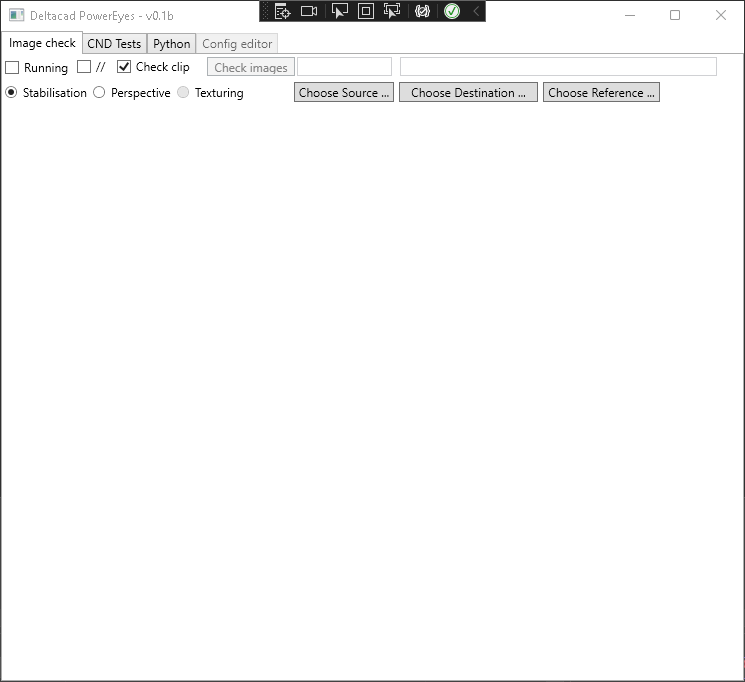
\includegraphics[height=5cm]{ressources/images/prototype.png}
    \caption{Prototype d'interface PowerEye}
\end{figure}
L'interface se compose de quatre modules: Image check, CND Tests, python et config editor. Il contient des méthodes d'application de de Template Matching pour la détection des pièces et des modèles d'entraînement pour les tests avec des ensembles de données.\\
Mais le fait est que l'interface prototype n'est pas suffisante pour inclure toutes les fonctionnalités envisagées par PowerEye. Par conséquent, ma principale contribution tout au long du stage a été la conception et le développement d'une nouvelle version de l'interface \texttt{PowerEye}. À la fin du stage, la nouvelle version de l'interface de powereye ressemblait à ceci. \\
\begin{figure}[h]
    \centering
    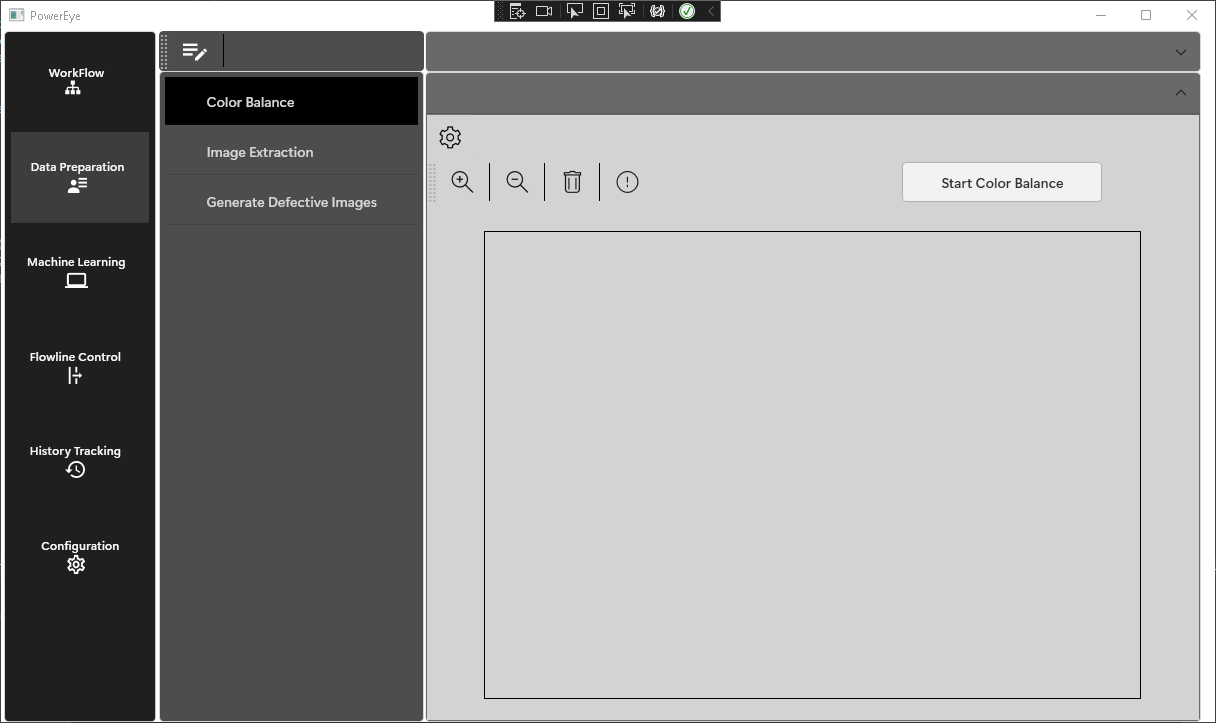
\includegraphics[height=6cm]{ressources/images/color_balance.png}
    \caption{Interface PowerEye redessinée}
\end{figure}
Il contient cinq modules : 
\begin{itemize}
    \item \textbf{Préparation des données (Data preparation): }Ce module permet d'extraire les contours des pièces de l'image et d'ajouter du bruit de perlin à l'image. 
    \item \textbf{Apprentissage automatique (machine learning): }Ce module est utilisé pour entraîner le modèle ckpt à partir de l'ensemble de données.
    \item \textbf{Contrôle de la chaîne d'assemblage (flowline control): } Ce module détecte si une pièce est qualifiée par Template Matching, et enregistre les données du résultat du test.
    \item \textbf{Interroger les données historiques  (History tracking): }Ce module interroge les données du fichier Excel par mots-clés.
    \item \textbf{Configuration des données globales (configuration): }Ce module affiche la configuration complète du logiciel en cours et l'importe par l'intermédiaire de fichiers de configuration.
\end{itemize}

En plus de la partie principale du logiciel, j'ai mis en place les fonctionnalités suivantes
\begin{itemize}
    \item Utilisation du cadre AOP pour afficher les actions de la couche applicative.
    \item Implémentation d'un script c\# qui s'exécute à partir d'une chaîne de caractères.
    \item Implémentation d'ajouts manuels de fonctionnalités existantes pour personnaliser le flux de travail.
\end{itemize}

Ce qui ci-dessus résume essentiellement toutes les contributions que j'ai apportées au cours de mon stage. Dans mon travail, j'ai conçu et développé le projet de manière indépendante en utilisant les exigences comme point de départ, et j'ai finalement bien accompli la tâche. 

\newpage
\section{Outils et technologies}
Tout au long de mon stage, j'ai travaillé avec les outils suivants : 
\begin{itemize}
    \item \textbf{Pour le développement :}
    \begin{itemize}
        \item \textit{Comme langage de programmation :} C\#, WPF.NET, C++, Python 
        \item \textit{Comme environnement de développement :} Microsoft Visual Studio, \gls{IDE}  complet pour les développeurs .NET et C++ sur Windows.
    \end{itemize}
    \item \textbf{Pour la bureautique :} \gls{LaTeX}, pour la rédaction de ce rapport. WebEx, pour les réunions de projet à distance
    \item \textbf{Pour la gestion des différentes versions du logiciel :} \gls{SmartSVN}, un système de gestion des versions.
\end{itemize}

Pour la réalisation du projet, j'ai utilisé les extensions suivantes :
\begin{itemize}
    \item \textbf{WPF-UI :} Extension pour modifier le style du contrôle
    \item \textbf{MahApps.Iconpacks :} Extension pour l'ajout d'icônes de boutons
    \item \textbf{Fody :} Extension pour la mise en œuvre du cadre aop
    \item \textbf{YamlDotNet :} Extension pour les modifications de l'édition yaml
\end{itemize}


\section{Validation de travaux}
La validation de mes travaux se déroulait lors de réunions avec l'équipe de projet. Comme le chef de projet ne travaille pas au même endroit que moi, nos réunions se passaient généralement à distance via le WebEx.

Au cours de la réunion, normalement, je commençais par présenter et démontrer l'état d'avancement de la tâche. Ensuite, le tuteur et le chef de projet discutaient avec moi des améliorations à apporter et planifient les tâches suivantes. le contenu de chaque réunion était enregistré par le chef de projet et m’était envoyé par e-mail après la réunion.

Cela me permet de partager mon point de vue sur le projet et me donne une idée claire de ce qui doit être fait a la phase actuel, ce qui améliore grandement mon efficacité et standardise mon travail.

\newpage
\section{Prise de recul}
\subsection{Intérêt de mon travail}
L'intérêt de mon travail pour l'équipe était de concevoir et développer une IHM plus aboutie que la précédente, migrer et améliorer les fonctionnalités développées précédemment. En outre, le cadre aop et le modèle de l'observateur sont plus propices à la maintenance de l'interface, et il existe un bon cadre général pour le développement du suivi. 

\subsection{Améliorations à envisager}
Mais tout comme le développement de nombreux logiciels connus nécessite beaucoup de polissage, le logiciel que j'ai développés au cours de mon stage de six mois n'étaient certainement pas parfait. Dans le développement futur du projet, les améliorations suivantes sont nécessaires.
\begin{itemize}
    \item Développer la fonctionnalité de certains modules et les intégrer dans l'interface.
    \item Extension de l'utilité de l'interface, par exemple par l'ajout de la touche de raccourci.
    \item Améliorer les fonctionnalités pour s'adapter aux différents produits de l'industrie.
\end{itemize}

\subsection{Réflexions sur l’impact de mon travail}
Selon moi, ma contribution permettra aux utilisateurs de simplifier le processus, de réduire le coût d'apprentissage de l'interface et de rendre la visualisation des résultats plus intuitive.
\end{document}
\grid